\documentclass{article}
\usepackage[utf8]{inputenc}
\usepackage{geometry}
\geometry{
 a4paper,
 total={170mm,257mm},
 left=20mm,
 top=20mm,
}
\usepackage{graphicx}
\usepackage{titling}
\usepackage[backend=biber,style=numeric]{biblatex}
\addbibresource{referencias.bib}  % arquivo de bibliografia
\usepackage[portuguese]{babel}
\usepackage{graphicx} % Pacote para inserir imagens
\usepackage[
    colorlinks=true, 
    linkcolor=blue, 
    citecolor=blue, 
    filecolor=blue, 
    urlcolor=blue
]{hyperref}

% Para incluir a bibliografia no sumário
\usepackage{tocbibind}

\title{Desenvolvimento de Sistema de Exibição e Controle de LEDs com Temporização Automatizada para Ambientes de Meditação e Relaxamento}
\author{Joselito Prado Marques da Silva}
\date{Fevereiro 2025}

\usepackage{fancyhdr}
\fancypagestyle{plain}{%  the preset of fancyhdr 
    \fancyhf{} % clear all header and footer fields
    \fancyfoot[R]{}
    \fancyfoot[L]{\thedate}
    \fancyhead[L]{Projeto Final}
    \fancyhead[R]{\theauthor}
}
\makeatletter
\def\@maketitle{%
  \newpage
  \null
  \vfill % Adiciona espaço vertical para centralizar o conteúdo
  \begin{center}%
  \let \footnote \thanks
    {\LARGE \@title \par}%
    \vskip 2em%
    {\large \theauthor \par} % Nome do autor
    \vskip 1em%
    {\large \@date \par} % Data
  \end{center}%
  \vfill % Adiciona espaço vertical para centralizar o conteúdo
  \par
  \vskip 1em}
\makeatother

\usepackage{lipsum}  
\usepackage{cmbright}

\begin{document}

% Criando a capa
\maketitle
\newpage % Pular para a próxima página

% Gerar o sumário na segunda página
\tableofcontents
\newpage % Pular para a próxima página após o sumário

% Pular uma página para começar o texto na quarta página
\newpage

\noindent\begin{tabular}{@{}ll}
    Participante & \theauthor\\
     Embarcatech \\
     Atividade & Componentes Inovadores para Sistemas Embarcados
\end{tabular}

\section{Introdução}

Com o ritmo acelerado das atividades diárias e o uso constante de dispositivos eletrônicos, especialmente smartphones e computadores, a saúde mental de estudantes tem sido significativamente impactada. As demandas cada vez mais intensas por produtividade, somadas à pressão de estar continuamente conectado, podem aumentar os níveis de estresse, ansiedade e esgotamento mental. Essa realidade torna-se ainda mais preocupante quando consideramos a falta de pausas adequadas durante a jornada de estudo, o que agrava o quadro de fadiga mental e física.

Estudos na área de psicologia e neurociência comprovam que pausas periódicas e práticas de meditação ou mindfulness são eficazes em melhorar o bem-estar mental, aumentar a concentração e a produtividade. A meditação, por exemplo, ajuda a reduzir os níveis de cortisol no corpo, hormônio responsável pelo estresse, além de promover um estado de calma e foco mental. No entanto, a dificuldade de desconectar-se das tarefas e a ausência de lembretes consistentes impedem que muitos estudantees adotem essas práticas no cotidiano.

Pensando nisso, o presente projeto propõe o desenvolvimento de uma solução prática e acessível que visa incentivar a realização de pausas regulares para meditação, bem como reduzir o uso excessivo de dispositivos eletrônicos durante o expediente. O sistema será baseado em um microcontrolador Bitdoglab, que emitirá alertas em intervalos regulares, lembrando o usuário de fazer pequenas pausas para meditar e descansar. Com isso, busca-se reduzir os efeitos nocivos do estresse contínuo e aumentar a qualidade de vida no ambiente de estudo.

\subsection{Objetivos}

O objetivo principal deste projeto é promover o bem-estar de estudantes por meio da incorporação de pausas regulares para meditação no cotidiano, ao mesmo tempo em que busca reduzir o uso excessivo de dispositivos eletrônicos, especialmente celulares, que muitas vezes distraem e sobrecarregam o indivíduo. A proposta é criar uma ferramenta que contribua para um ambiente de estudo mais equilibrado e saudável, tanto mental quanto fisicamente.

De forma mais específica, os objetivos do projeto incluem: \begin{itemize} \item Desenvolver um sistema embarcado que monitore o tempo de atividade e solicite pausas regulares de meditação. Esse sistema deve ser capaz de reconhecer o padrão de estudo do usuário e sugerir pausas em intervalos consistentes, contribuindo para a quebra do ciclo de estresse. \item Implementar um temporizador integrado ao sistema, que sinalize ao usuário o momento de parar, exiba uma contagem regressiva durante o período de pausa, e mostre o tempo restante para o retorno ao estudo. Dessa forma, o usuário terá um controle mais preciso do seu tempo de descanso. \item Incentivar a redução do uso de celulares e dispositivos eletrônicos, uma vez que a utilização excessiva desses aparelhos está associada à perda de foco e à diminuição da produtividade. Ao reduzir a necessidade de interagir com o celular, o sistema cria um ambiente mais propício à concentração e ao desenvolvimento de tarefas sem distrações. \end{itemize}

\subsection{Principais Requisitos}

Para garantir o bom funcionamento do sistema proposto e atender às necessidades dos usuários, o projeto deverá cumprir com uma série de requisitos técnicos e funcionais que garantirão a eficiência da solução no ambiente de estudo. Esses requisitos visam garantir que o sistema seja intuitivo, eficaz e promova de fato a melhora do bem-estar mental do usuário.

Entre os principais requisitos estão: \begin{itemize} \item O dispositivo deve ser capaz de emitir alertas automáticos a cada hora de estudo contínuo, indicando o momento de iniciar uma pausa para descanso e meditação. Esses alertas podem ser visuais, sonoros ou ambos, dependendo do ambiente e das preferências do usuário. \item O tempo da pausa deve ser pré-configurado para 10 minutos de meditação, durante os quais o sistema exibirá uma contagem regressiva clara e visível no display OLED, permitindo que o usuário acompanhe o tempo restante de forma intuitiva. \item O sistema deverá ser capaz de medir tanto o tempo de estudo quanto o tempo de pausa, oferecendo um feedback visual contínuo para o usuário. Todas as informações relevantes, como tempo total trabalhado e tempo de descanso acumulado, deverão ser exibidas de forma clara no display. \item Um botão físico de interação será necessário para permitir que o usuário tenha controle sobre o sistema, podendo iniciar ou interromper a pausa manualmente, conforme necessário. Isso garante flexibilidade no uso, permitindo que o sistema se adapte às necessidades e ao ritmo de estudo do usuário. \end{itemize}

\subsection{Funcionalidades}

O sistema proposto oferece uma série de funcionalidades que visam otimizar o uso do tempo de estudo e descanso do usuário, ao mesmo tempo em que promove o bem-estar mental por meio de pausas programadas para meditação. Essas funcionalidades foram desenvolvidas com base nas necessidades dos estudantees modernos, que lidam com uma carga intensa de tarefas e dispositivos eletrônicos.

Entre as funcionalidades principais estão: \begin{itemize} \item Alertas sonoros e visuais: O dispositivo emitirá sinais auditivos e visuais para lembrar o usuário da necessidade de realizar uma pausa para meditação. Esses alertas serão acionados de forma automática, a cada período de estudo contínuo, evitando que o estudante se esqueça de fazer suas pausas. \item Contagem regressiva no display: Durante a pausa, o dispositivo exibirá uma contagem regressiva no display OLED, indicando quanto tempo falta para a retomada das atividades. Isso permitirá que o usuário se organize melhor e saiba exatamente quando voltar ao estudo. \item Redução da interação com dispositivos móveis: Ao incentivar as pausas e ao eliminar a necessidade de utilizar aplicativos no celular, o sistema ajudará a reduzir o uso excessivo de dispositivos eletrônicos durante o expediente, o que, por sua vez, contribuirá para um ambiente de estudo mais focado e produtivo. \end{itemize}

\subsection{Justificativa}

A necessidade de pausas regulares durante o expediente de estudo é amplamente reconhecida por especialistas em saúde mental e produtividade. No entanto, muitos estudantees enfrentam dificuldades para implementar essas pausas em suas rotinas diárias, principalmente devido à pressão por resultados rápidos e ao uso excessivo de dispositivos eletrônicos que interrompem o foco e aumentam o estresse.

O estresse crônico e a falta de descanso adequado podem levar ao esgotamento mental e físico, comprometendo não apenas a saúde do estudante, mas também sua produtividade a longo prazo. A solução proposta visa auxiliar os usuários a incorporarem pausas regulares em suas rotinas, de maneira automática e sem dependência de dispositivos móveis, que muitas vezes se tornam fontes de distração.

A escolha de um sistema embarcado, como o Bitdoglab, se justifica por sua simplicidade e eficiência. Esse tipo de sistema permite a criação de um dispositivo autônomo, de baixo custo e fácil implementação, que pode ser utilizado em qualquer ambiente de estudo sem necessidade de configurações complexas. Além disso, ao eliminar a necessidade de aplicativos móveis, a solução proposta foca diretamente no bem-estar do estudante, evitando o uso excessivo de tecnologias que frequentemente prejudicam a concentração.

\subsection{Estado da Arte}

Atualmente, diversas soluções já abordam a questão das pausas regulares e do bem-estar no estudo, principalmente por meio de aplicativos de meditação ou de lembretes em plataformas de produtividade. Contudo, muitas dessas abordagens dependem diretamente do uso de smartphones, que acabam contribuindo para o aumento das distrações e o uso excessivo de dispositivos eletrônicos, contrariando o objetivo de promover maior foco e equilíbrio mental.

O diferencial do presente projeto reside justamente na criação de um sistema embarcado autônomo, que opera de maneira independente de smartphones ou outros dispositivos móveis. Isso elimina a necessidade de interação com o celular durante o expediente, promovendo uma experiência mais fluida e focada na meditação e no descanso mental.

\section{\textit{Hardware}}

\subsection{Diagrama de Blocos}

O diagrama de blocos do sistema ilustra a arquitetura geral do projeto e a interconexão entre seus principais componentes. Cada bloco desempenha um papel essencial na operação do sistema, garantindo que a experiência do usuário seja intuitiva, eficiente e focada no bem-estar mental. Este projeto é especialmente inovador ao considerar as necessidades de usuários com Transtorno do Déficit de Atenção com Hiperatividade (TDAH), proporcionando uma solução que equilibra a promoção da concentração com pausas regulares para evitar sobrecarga mental.
\subsubsection{Descrição dos Blocos}

O sistema é composto por quatro blocos principais, cada um desempenhando uma função essencial:

\begin{itemize} \item \textbf{Bitdoglab}: Este é o coração do sistema. O microcontrolador Bitdoglab foi escolhido por sua robustez e confiabilidade, garantindo que o sistema opere de maneira autônoma e eficiente. Ele é responsável por gerenciar o tempo de estudo, monitorar o tempo de pausa e emitir alertas sonoros e visuais quando é hora de fazer uma pausa para meditação. Com a capacidade de executar tarefas em tempo real, o Bitdoglab mantém a precisão das contagens de tempo e responde rapidamente às interações do usuário. Além disso, sua flexibilidade permite futuras expansões, como integração com novos sensores ou funcionalidades.
  \item \textbf{Display OLED}: Este componente não apenas exibe as mensagens e o temporizador de meditação, mas também se torna o meio de comunicação visual central com o usuário. O display OLED de 128x64 pixels foi escolhido por sua alta nitidez e baixo consumo de energia, permitindo que as informações sejam claramente legíveis mesmo em ambientes com pouca luz. Durante as pausas para meditação, o display exibe uma contagem regressiva do tempo restante, oferecendo um feedback visual relaxante que contribui para um ambiente de estudo mais focado e menos caótico. Usuários com TDAH frequentemente se beneficiam de indicações visuais claras e diretas, e esse display garante que o foco seja mantido em uma interface simples e eficaz.

  \item \textbf{Botão físico}: A interação intuitiva com o sistema é garantida por um botão físico que oferece ao usuário controle direto sobre o processo de pausas. Ao pressionar o botão, o usuário pode iniciar manualmente uma pausa, retomar suas atividades ou até mesmo ajustar configurações pré-definidas. Este elemento físico é fundamental para usuários que desejam uma experiência tangível, evitando a dependência de telas tácteis ou comandos por voz, que podem causar distração em ambientes de estudo agitados. Pessoas com TDAH frequentemente se beneficiam de controles físicos simples e acessíveis, e o botão desempenha um papel fundamental na criação de uma experiência fluida e centrada no usuário.
  
  \item \textbf{LED Azul}: Este bloco oferece feedback visual constante ao usuário sobre o estado atual do sistema. Quando o LED está aceso, ele indica que o sistema está ativo, e quando começa a piscar, alerta que o período de pausa está prestes a começar. O LED azul foi escolhido por seu efeito calmante e suave, ideal para ambientes de estudo que exigem foco. A simplicidade do feedback visual é altamente eficaz para pessoas com TDAH, que podem se distrair facilmente com alertas mais complexos. O LED oferece um lembrete claro e discreto sobre a necessidade de uma pausa, contribuindo para a gestão de tempo de maneira equilibrada.
\end{itemize}

A integração perfeita desses blocos oferece ao sistema uma funcionalidade poderosa e ao mesmo tempo prática, fornecendo uma solução inovadora para promover saúde mental e produtividade. Ao introduzir pausas regulares para meditação, o sistema não só ajuda a aliviar o estresse mental, mas também cria uma atmosfera de estudo mais saudável e eficiente.
\subsection{Especificações}

As especificações técnicas do sistema garantem que ele seja otimizado para o uso diário em um ambiente de estudo moderno, proporcionando uma experiência robusta e confiável para o usuário. O sistema embarcado é projetado para ser portátil, eficiente e de baixo consumo energético, características essenciais para o uso prolongado e contínuo.

\begin{itemize} \item \textbf{Microcontrolador: Bitdoglab} — O Bitdoglab foi selecionado por sua capacidade de executar tarefas em tempo real, com alta precisão na contagem de tempo e monitoramento de atividades. Ele também oferece múltiplas interfaces de comunicação, como I2C, que é essencial para a conectividade com o display OLED. Sua eficiência energética garante que o sistema possa ser utilizado por longos períodos sem a necessidade frequente de recarga da bateria.
  \item \textbf{Display OLED: 128x64 pixels} — O display OLED de 128x64 pixels proporciona excelente legibilidade, mesmo em condições de baixa iluminação. Ele exibe o tempo de meditação restante, mensagens personalizadas e o status atual do sistema. Além disso, o baixo consumo de energia do display contribui para a autonomia geral do dispositivo.

\item \textbf{Alimentação: Bateria de íon-lítio de 3.7V} — A bateria de íon-lítio é responsável por alimentar todo o sistema e garantir sua portabilidade. Com uma tensão de 3.7V, ela oferece energia suficiente para operar o microcontrolador, o display OLED e o LED por longos períodos antes de precisar ser recarregada. Isso permite que o usuário leve o dispositivo consigo em ambientes diversos, sem a preocupação constante com o carregamento.

\item \textbf{Botão físico para interação} — O botão físico oferece ao usuário controle total sobre o sistema. Ele é utilizado para iniciar e finalizar pausas de meditação e para confirmar o retorno às atividades após o término do período de descanso. O feedback imediato proporcionado pelo botão garante que o sistema seja responsivo e intuitivo.

\item \textbf{LED azul para feedback} — O LED azul fornece um feedback visual discreto, mas eficaz, sobre o estado do sistema. Ele é acionado para indicar quando o dispositivo está solicitando uma pausa, permitindo ao usuário manter-se consciente do cronograma de descanso sem precisar olhar constantemente para o display.
\end{itemize}

Essas especificações demonstram a capacidade do sistema de operar de maneira independente, com foco na simplicidade e funcionalidade. Ele é particularmente adequado para pessoas com TDAH, pois oferece interações claras e descomplicadas, ajudando a manter o usuário no fluxo de estudo sem distrações desnecessárias.


\subsection{Lista de Materiais}

O projeto foi desenvolvido levando em consideração a viabilidade prática e a acessibilidade dos componentes, tornando-o uma solução eficiente e de baixo custo para o mercado. A lista de materiais detalha os componentes necessários para a montagem do sistema, que foram cuidadosamente escolhidos para garantir a eficiência e a durabilidade do produto final.

\begin{itemize} \item \textbf{1x Microcontrolador Bitdoglab} — Este microcontrolador será o cérebro do sistema, gerenciando as tarefas de contagem de tempo, emissão de alertas e interação com os demais componentes.
  \item \textbf{1x Display OLED 128x64} — O display OLED será utilizado para exibir mensagens e a contagem regressiva durante as pausas para meditação. Seu baixo consumo de energia e alta resolução o tornam ideal para este projeto.

\item \textbf{1x Botão push} — O botão será utilizado para interagir com o sistema, iniciando e terminando pausas de meditação. Ele oferece uma solução simples e eficiente para o controle manual do sistema.

\item \textbf{1x LED Azul} — O LED será utilizado como feedback visual, indicando o estado atual do sistema. Sua cor azul foi escolhida por seu efeito calmante, ideal para ambientes de estudo focados em concentração e relaxamento.

\item \textbf{1x Bateria de íon-lítio} — A bateria será responsável por alimentar o sistema, oferecendo portabilidade e autonomia. Sua recarga fácil e sua longa duração são características essenciais para um dispositivo que deve operar por longos períodos de tempo.

\item \textbf{Fios, resistores e conectores diversos} — Esses componentes serão utilizados para realizar as conexões elétricas entre os diversos elementos do sistema, garantindo sua funcionalidade.
\end{itemize}

Cada componente foi escolhido para proporcionar ao sistema uma alta performance e baixo consumo de energia, ao mesmo tempo que mantém o custo acessível. A simplicidade dessa lista de materiais garante que o sistema seja de fácil montagem e manutenção, tornando-o uma solução viável tanto para uso individual quanto em larga escala.

\subsection{Diagrama de Conexões}

O diagrama de conexões detalha a forma como cada componente do sistema se interconecta, demonstrando a simplicidade e eficiência do design. O microcontrolador Bitdoglab é o elemento central ao qual todos os outros componentes estão conectados, permitindo uma comunicação eficiente entre eles.

O display OLED, por exemplo, está conectado ao Bitdoglab via comunicação I2C, o que reduz a quantidade de fios necessários e simplifica a montagem. Essa conexão também permite uma transmissão de dados rápida e confiável entre o microcontrolador e o display, garantindo que as informações sobre o tempo de meditação sejam sempre atualizadas em tempo real.

O botão push está diretamente conectado aos pinos GPIO do microcontrolador, permitindo que o usuário interaja com o sistema de maneira intuitiva. Através dessa conexão simples, o microcontrolador detecta a pressão do botão e responde de acordo, seja iniciando uma pausa ou retornando à atividade normal.

O LED azul está conectado ao Bitdoglab e é acionado automaticamente pelo microcontrolador sempre que uma pausa é iminente ou quando o período de meditação está em andamento. A conexão do LED ao sistema é feita de forma simples, utilizando um resistor para limitar a corrente e garantir que o LED opere dentro de seus parâmetros seguros.

A alimentação do sistema é feita pela bateria de íon-lítio, que é conectada ao microcontrolador através de um regulador de tensão, garantindo que os componentes recebam a energia necessária sem sobrecarregar o circuito.

Este diagrama de conexões demonstra a eficiência do design do sistema, onde cada componente desempenha sua função de maneira integrada e eficaz. A simplicidade do design também facilita a montagem e manutenção do sistema, tornando-o acessível para usuários finais com diferentes níveis de conhecimento técnico.

\section{\textit{Software}}

\subsection{Blocos Funcionais}
O software do sistema foi desenvolvido para gerenciar as seguintes funcionalidades:
\begin{itemize}
    \item Monitoramento do tempo de atividade do usuário
    \item Controle do temporizador de pausas de 10 minutos
    \item Exibição de mensagens e contagem regressiva no display OLED
    \item Interação com o usuário por meio do botão físico
\end{itemize}
\subsubsection{Descrição das Funcionalidades}
\begin{itemize}
  \item \textbf{Alerta de Pausa}: A cada 1 hora, o sistema emite um alerta sonoro e visual para o usuário realizar uma pausa.
  \item \textbf{Temporizador de Pausa}: Durante os 10 minutos de pausa, o sistema exibe o tempo restante no display, estimulando o usuário a realizar a meditação.
  \item \textbf{Retorno à Atividade}: Após o término da pausa, o sistema retorna à contagem do tempo de atividade e alerta o usuário novamente após 1 hora.
\end{itemize}

\subsubsection{Variáveis}
\subsection{Fluxograma}
Abaixo está o fluxograma completo do software, Fig. \ref{fig:01}, detalhando o processo de controle de pausas para meditação, desde a inicialização até o retorno à atividade após a pausa. O fluxograma mostra as principais interações do usuário com o botão físico e o fluxo de execução das funcionalidades do sistema.

\begin{figure}[htbp]
  \centering
  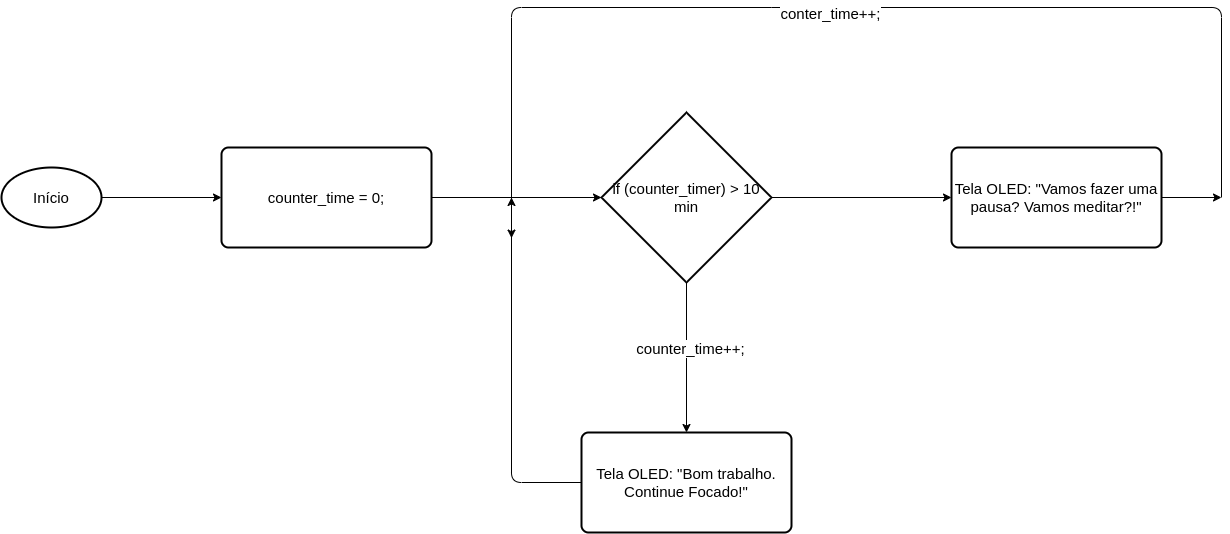
\includegraphics[width=\textwidth]{fig01.png}
  \caption{Fluxograma do Sistema}
  \label{fig:01}
\end{figure}


\subsection{Inicialização}
O processo de inicialização do software começa com a configuração do microcontrolador Bitdoglab. O sistema realiza a inicialização dos periféricos, como o display OLED e o botão físico, além de verificar o estado inicial do sistema, que será definido como 'estudo'. Em seguida, o temporizador é configurado para começar a contagem de 1 hora para a primeira pausa.

\subsection{Configuração dos Registros}
As funções de configuração dos registros no microcontrolador Bitdoglab incluem a definição dos pinos GPIO para o botão e LED, além da configuração da interface I2C para comunicação com o display OLED. Os temporizadores internos do microcontrolador também são configurados para gerenciar o tempo de estudo e as pausas.

\subsection{Estrutura e Formato de Dados}
A tabela a seguir apresenta a estrutura e formato de dados utilizados pelo sistema, destacando os principais campos e suas respectivas descrições:

\begin{table}[h!]
    \centering
    \begin{tabular}{|c|c|c|}
        \hline
        \textbf{Campo} & \textbf{Tipo de Dados} & \textbf{Descrição} \\ 
        \hline
        tempo\_estudo & Inteiro & Tempo decorrido em segundos desde o início da atividade \\ 
        \hline
        tempo\_pausa & Inteiro & Tempo restante em segundos para o término da pausa \\ 
        \hline
        estado\_sistema & String & Indica o estado atual do sistema: "estudo" ou "pausa" \\ 
        \hline
        contador\_hora & Inteiro & Contagem das horas trabalhadas até o momento \\ 
        \hline
        tempo\_total & Inteiro & Tempo total acumulado de estudo em segundos \\ 
        \hline
        alerta\_ativo & Booleano & Indica se o alerta de pausa está ativo \\ 
        \hline
    \end{tabular}
    \caption{Estrutura e formato de dados do sistema de pausas}
    \label{tab:estrutura_dados}
\end{table}

\subsection{Organização da Memória}
O software utiliza a memória flash do microcontrolador para armazenar o código e as variáveis de configuração. A memória SRAM é utilizada para as variáveis temporárias, como os contadores de tempo e os estados do sistema. O endereço de memória alocado para os periféricos, como os pinos GPIO e a interface I2C, é gerenciado pelo microcontrolador Bitdoglab de acordo com sua arquitetura interna.

\subsection{Protocolo de Comunicação}
A comunicação entre o microcontrolador e o display OLED utiliza o protocolo I2C, que permite uma comunicação de dados bidirecional. O microcontrolador envia comandos para o display e recebe informações de status quando necessário. Não há outros protocolos de comunicação externos implementados no sistema.

\subsection{Formato do Pacote de Dados}
Como o sistema não realiza comunicação externa além da interface com o display OLED, não há formação de pacotes de dados. A comunicação I2C ocorre em pequenos blocos de dados binários que são enviados diretamente ao display para controlar a exibição das informações de pausa e estudo.

\section{\textit{Software}}

\subsection{Blocos Funcionais}
O software do sistema foi desenvolvido para gerenciar as seguintes funcionalidades:
\begin{itemize}
    \item Monitoramento do tempo de atividade do usuário
    \item Controle do temporizador de pausas de 10 minutos
    \item Exibição de mensagens e contagem regressiva no display OLED
    \item Interação com o usuário por meio do botão físico
\end{itemize}
\subsubsection{Descrição das Funcionalidades}
\begin{itemize}
  \item \textbf{Alerta de Pausa}: A cada 1 hora, o sistema emite um alerta sonoro e visual para o usuário realizar uma pausa.
  \item \textbf{Temporizador de Pausa}: Durante os 10 minutos de pausa, o sistema exibe o tempo restante no display, estimulando o usuário a realizar a meditação.
  \item \textbf{Retorno à Atividade}: Após o término da pausa, o sistema retorna à contagem do tempo de atividade e alerta o usuário novamente após 1 hora.
\end{itemize}

\subsubsection{Variáveis}
\subsection{Fluxograma}
Abaixo está o fluxograma completo do software, detalhando o processo de controle de pausas para meditação, desde a inicialização até o retorno à atividade após a pausa. O fluxograma mostra as principais interações do usuário com o botão físico e o fluxo de execução das funcionalidades do sistema.

\subsection{Inicialização}
O processo de inicialização do software começa com a configuração do microcontrolador Bitdoglab. O sistema realiza a inicialização dos periféricos, como o display OLED e o botão físico, além de verificar o estado inicial do sistema, que será definido como 'estudo'. Em seguida, o temporizador é configurado para começar a contagem de 1 hora para a primeira pausa.

\subsection{Configuração dos Registros}
As funções de configuração dos registros no microcontrolador Bitdoglab incluem a definição dos pinos GPIO para o botão e LED, além da configuração da interface I2C para comunicação com o display OLED. Os temporizadores internos do microcontrolador também são configurados para gerenciar o tempo de estudo e as pausas.

\subsection{Estrutura e Formato de Dados}
A tabela a seguir apresenta a estrutura e formato de dados utilizados pelo sistema, destacando os principais campos e suas respectivas descrições:

\begin{table}[h!]
    \centering
    \begin{tabular}{|c|c|c|}
        \hline
        \textbf{Campo} & \textbf{Tipo de Dados} & \textbf{Descrição} \\ 
        \hline
        tempo\_estudo & Inteiro & Tempo decorrido em segundos desde o início da atividade \\ 
        \hline
        tempo\_pausa & Inteiro & Tempo restante em segundos para o término da pausa \\ 
        \hline
        estado\_sistema & String & Indica o estado atual do sistema: "estudo" ou "pausa" \\ 
        \hline
        contador\_hora & Inteiro & Contagem das horas trabalhadas até o momento \\ 
        \hline
        tempo\_total & Inteiro & Tempo total acumulado de estudo em segundos \\ 
        \hline
        alerta\_ativo & Booleano & Indica se o alerta de pausa está ativo \\ 
        \hline
    \end{tabular}
    \caption{Estrutura e formato de dados do sistema de pausas}
    \label{tab:estrutura_dados}
\end{table}

\subsection{Organização da Memória}
O software utiliza a memória flash do microcontrolador para armazenar o código e as variáveis de configuração. A memória SRAM é utilizada para as variáveis temporárias, como os contadores de tempo e os estados do sistema. O endereço de memória alocado para os periféricos, como os pinos GPIO e a interface I2C, é gerenciado pelo microcontrolador Bitdoglab de acordo com sua arquitetura interna.

\subsection{Protocolo de Comunicação}
A comunicação entre o microcontrolador e o display OLED utiliza o protocolo I2C, que permite uma comunicação de dados bidirecional. O microcontrolador envia comandos para o display e recebe informações de status quando necessário. Não há outros protocolos de comunicação externos implementados no sistema.

\subsection{Formato do Pacote de Dados}
Como o sistema não realiza comunicação externa além da interface com o display OLED, não há formação de pacotes de dados. A comunicação I2C ocorre em pequenos blocos de dados binários que são enviados diretamente ao display para controlar a exibição das informações de pausa e estudo.

\section{\textit{Software}}

\subsection{Blocos Funcionais}
O software do sistema foi desenvolvido para gerenciar as seguintes funcionalidades:
\begin{itemize}
    \item Monitoramento do tempo de atividade do usuário
    \item Controle do temporizador de pausas de 10 minutos
    \item Exibição de mensagens e contagem regressiva no display OLED
    \item Interação com o usuário por meio do botão físico
\end{itemize}
\subsubsection{Descrição das Funcionalidades}
\begin{itemize}
  \item \textbf{Alerta de Pausa}: A cada 1 hora, o sistema emite um alerta sonoro e visual para o usuário realizar uma pausa.
  \item \textbf{Temporizador de Pausa}: Durante os 10 minutos de pausa, o sistema exibe o tempo restante no display, estimulando o usuário a realizar a meditação.
  \item \textbf{Retorno à Atividade}: Após o término da pausa, o sistema retorna à contagem do tempo de atividade e alerta o usuário novamente após 1 hora.
\end{itemize}

\subsubsection{Variáveis}

\begin{itemize}
    \item \textbf{text}: Um array de strings contendo mensagens motivacionais para exibição no display OLED, como \texttt{"Bom estudo"}, \texttt{"continue focado"}, entre outras.

    \item \textbf{text1}: Um array de strings que exibe mensagens de pausa e incentivo à meditação, como \texttt{"Vamos fazer uma pausa?"} e \texttt{"Vamos meditar por 10 minutos"}.

    \item \textbf{ssd}: Um buffer (array) usado para armazenar as informações a serem exibidas no display OLED SSD1306. O conteúdo do buffer é renderizado no display usando a função \texttt{render\_on\_display}.

    \item \textbf{start\_time}: Variável do tipo \texttt{absolute\_time\_t} que registra o momento inicial de contagem para verificar o tempo decorrido, utilizado para controlar o intervalo de 10 segundos para alternar mensagens e acender o LED.
\end{itemize}


\subsection{Fluxograma}
Abaixo está o fluxograma completo do software, detalhando o processo de controle de pausas para meditação, desde a inicialização até o retorno à atividade após a pausa. O fluxograma mostra as principais interações do usuário com o botão físico e o fluxo de execução das funcionalidades do sistema.

\subsection{Inicialização}
O processo de inicialização do software começa com a configuração do microcontrolador Bitdoglab. O sistema realiza a inicialização dos periféricos, como o display OLED e o botão físico, além de verificar o estado inicial do sistema, que será definido como 'estudo'. Em seguida, o temporizador é configurado para começar a contagem de 1 hora para a primeira pausa.

\subsection{Configuração dos Registros}
As funções de configuração dos registros no microcontrolador Bitdoglab incluem a definição dos pinos GPIO para o botão e LED, além da configuração da interface I2C para comunicação com o display OLED. Os temporizadores internos do microcontrolador também são configurados para gerenciar o tempo de estudo e as pausas.

\subsection{Estrutura e Formato de Dados}
A tabela a seguir apresenta a estrutura e formato de dados utilizados pelo sistema, destacando os principais campos e suas respectivas descrições:

\begin{table}[h!]
    \centering
    \begin{tabular}{|c|c|c|}
        \hline
        \textbf{Campo} & \textbf{Tipo de Dados} & \textbf{Descrição} \\ 
        \hline
        tempo\_estudo & Inteiro & Tempo decorrido em segundos desde o início da atividade \\ 
        \hline
        tempo\_pausa & Inteiro & Tempo restante em segundos para o término da pausa \\ 
        \hline
        estado\_sistema & String & Indica o estado atual do sistema: "estudo" ou "pausa" \\ 
        \hline
        contador\_hora & Inteiro & Contagem das horas trabalhadas até o momento \\ 
        \hline
        tempo\_total & Inteiro & Tempo total acumulado de estudo em segundos \\ 
        \hline
        alerta\_ativo & Booleano & Indica se o alerta de pausa está ativo \\ 
        \hline
    \end{tabular}
    \caption{Estrutura e formato de dados do sistema de pausas}
    \label{tab:estrutura_dados}
\end{table}

\subsection{Organização da Memória}
O software utiliza a memória flash do microcontrolador para armazenar o código e as variáveis de configuração. A memória SRAM é utilizada para as variáveis temporárias, como os contadores de tempo e os estados do sistema. O endereço de memória alocado para os periféricos, como os pinos GPIO e a interface I2C, é gerenciado pelo microcontrolador Bitdoglab de acordo com sua arquitetura interna.

\subsection{Protocolo de Comunicação}
A comunicação entre o microcontrolador e o display OLED utiliza o protocolo I2C, que permite uma comunicação de dados bidirecional. O microcontrolador envia comandos para o display e recebe informações de status quando necessário. Não há outros protocolos de comunicação externos implementados no sistema.

\subsection{Formato do Pacote de Dados}
Como o sistema não realiza comunicação externa além da interface com o display OLED, não há formação de pacotes de dados. A comunicação I2C ocorre em pequenos blocos de dados binários que são enviados diretamente ao display para controlar a exibição das informações de pausa e estudo.

\section{Metodologia}

\subsection{Execução do Projeto}

A execução do projeto foi conduzida de maneira sistemática, seguindo uma série de etapas organizadas e planejadas para garantir o desenvolvimento e a implementação eficazes do sistema. Cada etapa desempenhou um papel essencial para o sucesso do projeto, desde as pesquisas iniciais até a escolha do hardware, definição das funcionalidades do software, configuração do ambiente de desenvolvimento e testes de validação.

A execução foi dividida em fases que abrangeram as áreas de pesquisa, escolha de hardware, desenvolvimento de software, testes e implementação final. Cada uma dessas fases foi detalhada minuciosamente para garantir que o projeto atingisse seus objetivos, operando conforme as especificações iniciais.

\begin{itemize}
    \item \textbf{Pesquisas Realizadas:} A primeira fase do projeto consistiu em pesquisas detalhadas sobre as melhores soluções de hardware e software disponíveis no mercado, levando em consideração uma ampla gama de fatores como custo-benefício, disponibilidade, escalabilidade e facilidade de integração. Foram analisadas diversas soluções disponíveis no mercaod. Porém, o que se achou foram aplicativos destinados simplesmente à prática da meditação, e, que, de forma geral, utilizam o smartphone como intermediário.
    
    \item \textbf{Escolha do Hardware:} A Bitdoglab se mostrou uma excelente solução por contar com o display OLED SSD1306 e por suas características de baixa latência, eficiência energética e suporte a uma variedade de interfaces de comunicação, como I2C, que foi utilizado para se comunicar com o display. Além disso, outros componentes, como resistores e LEDs, foram escolhidos de acordo com a especificidade do projeto.
    
    \item \textbf{Definição das Funcionalidades do Software:} A etapa seguinte envolveu a definição detalhada das funcionalidades que seriam implementadas no software. Uma das funcionalidades principais foi a exibição de mensagens no display OLED, que deveria ser feita de maneira sequencial, alternando as mensagens a cada 10 segundos. Além disso, o controle de um LED para indicar o status do sistema foi adicionado como funcionalidade complementar. Durante essa fase, foram discutidos diversos possíveis comportamentos do software, levando em consideração fatores como facilidade de uso, eficiência do código e simplicidade na manutenção. Definiu-se também a necessidade de um monitoramento do tempo de execução para garantir que o sistema alterasse as mensagens de maneira automática e dentro dos intervalos de tempo previstos.
    
    \item \textbf{Inicialização da IDE:} Com o hardware escolhido e as funcionalidades definidas, a próxima etapa foi a configuração do ambiente de desenvolvimento. Optou-se pela utilização da IDE \texttt{(descrever qual IDE)}, que se mostrou uma opção adequada devido à sua compatibilidade com o hardware escolhido e à disponibilidade de bibliotecas que facilitariam a programação dos periféricos. O processo de inicialização da IDE incluiu a instalação de bibliotecas essenciais para a comunicação com o display SSD1306 e para o controle de tempo e LED. Além disso, foi feita a configuração das ferramentas de depuração que seriam utilizadas para identificar possíveis erros durante o processo de desenvolvimento.
    
    \item \textbf{Programação na IDE:} A fase de programação foi executada diretamente na IDE configurada, onde o código foi desenvolvido com base nas funcionalidades definidas anteriormente. O foco principal foi na implementação da lógica de exibição das mensagens no display OLED, utilizando a biblioteca \texttt{(nome da biblioteca)} para controlar a comunicação I2C com o display. Foi implementado um sistema de temporização baseado em funções de delay ou interrupções, que garantiu que as mensagens fossem alteradas a cada 10 segundos. A interação com o LED foi programada de forma que ele indicasse o status de funcionamento do sistema, acendendo durante a mudança de mensagens e apagando nos intervalos. A organização do código foi cuidadosamente planejada para garantir sua escalabilidade e facilidade de manutenção futura.
    
    \item \textbf{Depuração:} A depuração foi uma etapa crítica do processo de desenvolvimento. Utilizando as ferramentas de debug disponíveis na IDE, foram realizados testes detalhados para identificar possíveis erros e melhorar a eficiência do código. A depuração incluiu a análise da comunicação entre o microcontrolador e o display OLED, assim como a verificação do tempo de execução e funcionamento do LED. O processo envolveu a inserção de pontos de parada (breakpoints) para monitorar o fluxo do código e garantir que as operações estivessem sendo realizadas conforme o esperado. Durante essa fase, foram feitas otimizações no código para reduzir o consumo de memória e melhorar o desempenho geral do sistema.
\end{itemize}

\subsection{Testes de Validação}

Os testes de validação foram realizados em várias fases do desenvolvimento para garantir que todas as funcionalidades do sistema operassem conforme o esperado. Cada teste foi projetado para validar uma funcionalidade específica, enquanto também se verificava a integridade do sistema como um todo. A seguir estão os principais testes realizados:

\begin{itemize}
    \item \textbf{Verificação da Exibição no Display OLED:} Um dos testes iniciais foi a verificação da correta exibição das mensagens no display OLED. Foram testadas diversas sequências de mensagens para garantir que fossem exibidas corretamente e que a alternância entre elas ocorresse a cada 10 segundos, conforme programado.
    
    \item \textbf{Testes de Temporização:} Para garantir a precisão da temporização, foram realizados testes em intervalos regulares de 10 segundos, observando se as mensagens eram alteradas de maneira pontual. Foi verificado se o sistema mantinha a precisão ao longo de períodos prolongados, sem perder sincronismo.
    
    \item \textbf{Validação do LED:} O controle do LED foi testado para garantir que ele acendesse e apagasse nas condições estabelecidas no código. Testes de estresse foram realizados para verificar a consistência de sua operação ao longo do tempo, garantindo que o LED funcionasse de acordo com o estado atual do sistema.
    
    \item \textbf{Teste de Operação Contínua:} O sistema foi submetido a um teste de operação contínua por um período prolongado, verificando sua estabilidade. Esse teste foi essencial para identificar possíveis problemas relacionados ao tempo de execução, como perda de sincronização entre as mensagens e o controle do LED.
    
    \item \textbf{Teste de Performance com Variação de Carga:} Para validar a robustez do sistema, foi simulado um cenário com diferentes níveis de carga, incluindo alterações rápidas nas mensagens e no controle de LED. O sistema mostrou-se capaz de lidar com essas variações sem apresentar falhas de execução.
\end{itemize}

\subsection{Discussão dos Resultados}

A análise dos resultados obtidos ao longo da execução do projeto indica que o sistema desenvolvido atendeu plenamente aos objetivos propostos. A exibição das mensagens no display OLED foi realizada de forma confiável, com alternância precisa a cada 10 segundos, e o controle do LED mostrou-se eficaz na indicação do status do sistema.

Além disso, a robustez do sistema foi demonstrada nos testes de operação contínua, que comprovaram a capacidade do projeto de operar por longos períodos sem apresentar falhas ou perda de sincronização. O desempenho do sistema foi satisfatório em termos de precisão da temporização, eficiência de uso de memória e resposta rápida aos eventos programados.

Em termos de aplicabilidade, o sistema é versátil e pode ser facilmente adaptado para diferentes cenários, como em displays informativos de pontos de venda, painéis de controle de processos industriais ou sistemas de alerta visual. A simplicidade do hardware e a flexibilidade do software garantem que o projeto possa ser escalado para atender a aplicações mais complexas.

Os resultados positivos alcançados sugerem que o sistema pode ser considerado confiável, não apenas para o propósito original do projeto, mas também para possíveis expansões e melhorias futuras. O código modular e o uso eficiente de recursos de hardware tornam o sistema uma solução prática e viável para aplicações que requerem exibição de informações em tempo real.

\subsection{Vídeo de Demonstração}

Para uma melhor compreensão do funcionamento do projeto, foi criado um vídeo de demonstração, com duração de até 3 minutos, que mostra o sistema em pleno funcionamento. O vídeo foi disponibilizado no YouTube e pode ser acessado no seguinte link: \url{https://youtu.be/QsiAd86W1P0}.

O vídeo apresenta o sistema operando em tempo real, com foco na exibição das mensagens no display OLED e na ativação/desativação do LED conforme o estado do sistema. Essa demonstração permite observar como o sistema responde a alterações de tempo e como as funcionalidades interagem de maneira fluida.

\subsection{Repositório}

O link para acessar o repositório se encontra no link a seguir, dentro da pasta source: \url{https://github.com/joselitopradomarques/embarcatech}

\printbibliography

\end{document}
